\chapter{Comparing transitivity across languages}\label{chapter:transitivity}

\section{From transitivity categories to transitivity ratios}

It is logical when doing cross-linguistic comparison to start with simpler metrics and features before developing to more complex ones. On the one hand, it is true that regardless of how we approach the task of verb classification, i.e., to categorize the verbs of a language into verb classes according to their syntacto-semantic properties and behavior, we would expect to arrive at fine-grained verb classes à la \citet{levin1993} in the end. On the other hand, such an expectation does not render obsolete the more basic distinctions like that of verb \textit{transitivity}. In part, this is due to their utility as convenient starting points of comparison for verbs within a language, but their simplicity also translates to being more cross-lingually valid bases of typological comparison. 

This first experiment deals with metrics of \textit{transitivity}, i.e., the ability of a verb to take one or more objects. It is surely a more familiar and intuitive concept as compared to the finer-grained metrics of valency to follow in the experiments in the next chapter. In traditional grammars, a basic binary distinction is made between \textit{intransitive} verbs, which take only a subject and no objects and \textit{transitive} verbs, which take one or more objects. Additional categories, some overlapping, make finer distinctions, such as \textit{ditransitive} verbs (those taking two objects), \textit{ambitransitive} verbs (those that can be used both transitively and intransitively), etc.

I focus here on the simple distinction between transitive and intransitive verbs, but, hewing to a functional and quantitative outlook, find that binary categories do not sufficiently capture the nuances of verb use. An example illustrating why comes from the study of near-synonyms: \citep{biber1998}, an early corpus linguistics study, compares the English verbs \textit{begin} and \textit{start} in the British National Corpus (BNC). At first glance, English appears to have provided us with two verbs that are not only semantically synonymous but share valency properties as well, as they can both be used in transitive and intransitive constructions:

\begin{exe}
\ex\label{example-begin_start}
  \begin{xlist}
  \ex{I had better issue a survival kit before we \textit{start}/\textit{begin}.\\ \strut\hfill \textbf{intransitive}}
  \ex{Then they \textit{started}/\textit{began} the quota system.\\ \strut\hfill \textbf{transitive with noun phrase}}
  \ex{They'd \textit{started}/\textit{begun} leaving before I arrived.\\ \strut\hfill \textbf{transitive with \textit{-ing} clause}}
  \ex{One of the wheels had \textit{started}/\textit{begun} to wobble.\\ \strut\hfill \textbf{transitive with \textit{to} clause}}
  \end{xlist}
\end{exe}

This however belies their different usage patterns as observed in the BNC: while both uses are clearly grammatical for both verbs, \textit{begin} is used more often in a transitive frame than \textit{start} across different genres in the BNC: in fiction, 78\% of \textit{begin} occurrences (196/250) are with various transitive patterns vs. only 60\% for \textit{start} (149/250); transitive uses are less frequent in academic texts in general but the observation of relatively higher transitivity for \textit{begin} still holds (57\% vs. 36\%, or 110/192 vs. 51/142).

To capture such differences in levels of transitivity, I propose measuring \textbf{transitivity ratios} based on language corpora, defined as the percentage of verb instances that are transitive. The verbs of a language can then be thought of as on a spectrum of transitivity, with strictly intransitive verbs on the one end, strictly transitive verbs on the opposite end, and all other verbs\footnote{Note that not all of them are ambitransitive verbs, as the approach here is only concerned with the surface realization of transitivity. In particular, this means instances of pro-drop of objects are counted as intransitive, where some would argument for a null object analysis instead.} somewhere in between.

\section{Experiment 1: Transitivity at token and lexeme levels}\label{sec:exp1}

\subsection{Introduction}

Necessarily then, and in contrast with transitivity categories, any values are calculated on an \textit{ad hoc} basis in a given corpus. Unless we expect the corpus to be a representative sample of all language use in that language, which is certainly not the case for the UD corpora used here, the absolute values of these ratios at a lexeme-level cannot be directly interpreted. Instead, intralinguistic analysis will take the form of analyzing the distribution of verbs according to their observed transitivity ratios. I take on an additional assumption, that the corpus would reflect the general tendency towards (in-)transitivity of the language, if too piecemeal for individual verbs, which justifies the cross-lingual comparison of transitivity ratios at a token-level as well.

\subsection{Methodology}

The UD annotation scheme facilitates the investigation of transitivity at lexeme- and token-levels, as the relevant dependency relations \textsc{nsubj} and \textsc{obj} mark respectively the first and second core arguments of a verb with their typical syntactic roles as subject and object. This is defined without respect to specific cases (even though typically the nominative and the accusative in languages with a case system) or semantic roles (even though they would typically be the proto-agent and the proto-patient) in an effort to avoid \textit{a priori} categories to the extent possible. The renaming of the \textsc{dobj} relation to \textsc{obj}, among the changes introduced by UD v2 \citep{nivre2020}, reflects the same laudable effort.

Despite the typologically sound UD dependency relation annotations, arriving at a clear definition of transitivity ratio in the UD context is still not trivial upon close examination. In fact, I consider four different definitions of a quantitative transitivity ratio within the UD annotation scheme here:

\begin{enumerate}
    \item the ratio of verb instances with both \textsc{nsubj} and \textsc{obj} dependents, as compared to verb instances with an \textsc{nsubj} dependent
    \item the ratio of verb instances with an \textsc{obj} dependent, as compared to verb instances with an \textsc{nsubj} dependent
    \item the ratio of verb instances with an \textsc{obj} dependent, as compared to all verb instances
    \item the ratio of verb instances with an \textsc{obj} dependent, as compared to verb instances with either an \textsc{nsubj} or an \textsc{obj} dependent
\end{enumerate}

Def. 1 is an attempt at enforcing a definition of the transitive object as the \textit{second} core argument of the verb by excluding from calculation instances where the first core argument (i.e., subject) is not realized. This turns out counterproductive for two reasons. Firstly, this does not sit well with the core definition on transitivity, as instances of verb use where the subject is not expressed should not count against the fact that the verb is taking a transitive object; secondly, this is undesirable in practice when accounting for typological variations, as the metric would be biased against pro-drop languages that drops subject pronouns more often than objects such as Spanish and Catalan.

Revising def. 1 and dropping the requirement in the numerator for verbs to have an \textsc{nsubj} dependent gives us def. 2. However, this is not sufficient, as the opposite problem surfaces, where subject-dropping languages are likely to have a smaller denominator, resulting in a high transitivity ratio that is not representative. Def. 3 drops the \textsc{nsubj} requirement from the denominator as well. This still faces problems, as verb instances where both subject and object are dropped would affect the denominator, and such usage, e.g., non-predicative usage of verbs, is unlikely to be equally frequent in different languages and would therefore interfere with the cross-lingual comparability of our transitivity ratio focusing on argument structure of verb predicates. Taking all these potential drawbacks into consideration, we arrive at def. 4 with the number of verb instances with either an \textsc{nsubj} or an \textsc{obj} dependent in the denominator. 

\begin{table}[ht]
    \centering
    \begin{tabularx}{0.5\textwidth}{cX}
    {\#} & \textbf{Definition} \\
    \hline
    1&$[+\textsc{nsubj}, +\textsc{obj}]/ [+\textsc{subj}]$ \\
    2&$[+\textsc{obj}] / [+\textsc{nsubj}]$  \\
    3&$[+\textsc{obj}] / [\pm\textsc{nsubj}, \pm\textsc{obj}]$\\
    4&$[+\textsc{obj}] / [+\textsc{nsubj}] \text{ or } [+\textsc{obj}]$
    \end{tabularx}
    \caption{Potential definitions of transitivity ratio considered in §\ref{sec:exp1}, represented with feature matrices}\label{tab:transitivity-defs}
\end{table} 

While there is a strong case for Def. 4 being the most principled definition, I nevertheless implement all four definitions in this experiment to empirically verify the intuitions. They are also represented with feature matrices in Tab.~\ref{tab:transitivity-defs} for quick reference.

\subsection{Results and discussion}\label{subsec:transitivity-lexicon}

Transitivity ratio statistics for each verb lexeme based on the definitions are first compiled. From there, per-language statistics that will become the basis for our cross-lingual comparison are computed: I calculate the lexeme-level and token-level transitivity ratios for each language, respectively the arithmetic mean of the lexeme transitivity ratios and the mean of lexeme transitivity ratios weighted by the frequency of the lexeme. In addition to the transitivity ratio metrics, an additional metric, percentage of transitive verbs, i.e., the percentage of verbs in the observed lexicon that are not strictly intransitive (defined as never observed to take an \textsc{obj}), is calculated for comparison purposes, as it should correspond better with the traditional binary distinction between transitive and intransitive verbs.

I perform the experiment on the selected subset of UD data as described in §\ref{sec:data_selection}. For the analysis, I include only languages with at least 50 observed verb lexemes (69 out of 79 languages); the full results from the experiments can be found in the accompanying data and appendices. 

\begin{table}[ht]{}
    \centering
    \small
    \begin{tabularx}{\textwidth}{lXXX}
      \toprule
      def. & lexeme tr.,\newline token tr. & tr. verb \%,\newline lexeme tr. & tr. verb \%,\newline token tr. \\
      \midrule
      1 & $\rho(54)=.83, p=.000$ & $\rho(54)=.61, p=.000$ & $\rho(54)=.70, p=.000$ \\
      2 & $\rho(54)=.81, p=.000$ & $\rho(54)=-.17, p=.221$ & $\rho(54)=-.03, p=.817$ \\
      3 & $\rho(54)=.77, p=.000$ & $\rho(54)=.64, p=.000$ & $\rho(54)=.73, p=.000$ \\
      4 & $\rho(54)=.87, p=.000$ & $\rho(54)=.61, p=.000$ & $\rho(54)=.61, p=.000$ \\
      \bottomrule
    \end{tabularx}
    \caption{Spearman's rank correlation between the transitivity metrics}\label{tab:transitivity_spearmanr} 
\end{table}  

To compare between the different definitions of transitivity, we compute Spearman's rank correlations between the lexeme- and token-level means of transitivity ratios according to each of our four definitions, as well as between the transitive verb percentage and each of them. The correlation statistics are listed in Tab.~\ref{tab:transitivity_spearmanr}. We observe overall strong correlations between the mean transitivity ratios at lexeme and token levels for all four definitions, with the highest observed for definition 4 ($\rho(67)=.88, p=.000$) and lowest observed for definition 1 ($\rho(67)=.76, p=.000$). The strong correlation is not surprising as we have no reason to expect the more frequent verbs to behave differently from the less frequent verbs with regard to transitivity ratios. This can also be confirmed by correlation tests between verb frequency and verb transitivity ratios for each language, which show no strong correlation (Spearman's $\rho$ between all languages).

The correlation statistics between the transitive verb percentages and the transitivity ratios are more revealing. Definition 2 is eliminated as it does not show statistically significant correlation at lexeme level ($\rho(67)=.20, p=.106$) and weak correlation at token level ($\rho(67)=.27, p=.025$). Of the other three, only definition 4, our \textit{a priori} favorite, show strong correlations at both token and lexeme levels ($\rho(67)=.70, p=.000$ and $\rho(67)=.72, p=.000$, respectively). 

While this comparison is not conclusive, it indicates that definition 4 provides more robust results across the levels of measurement, providing circumstantial support to our \textit{a priori} determination. For the sake of simplicity, the rest of the experiment are reported relying on the transitivity ratios as defined in definition 4. 

Further intralinguistic analyses are done by plotting histograms of the distributions of verbs among the transitivity ratios in different languages, as shown in Fig.~\ref{fig:verb_dist_transitivity}.

\begin{sidewaysfigure}[ht]
  \centering
  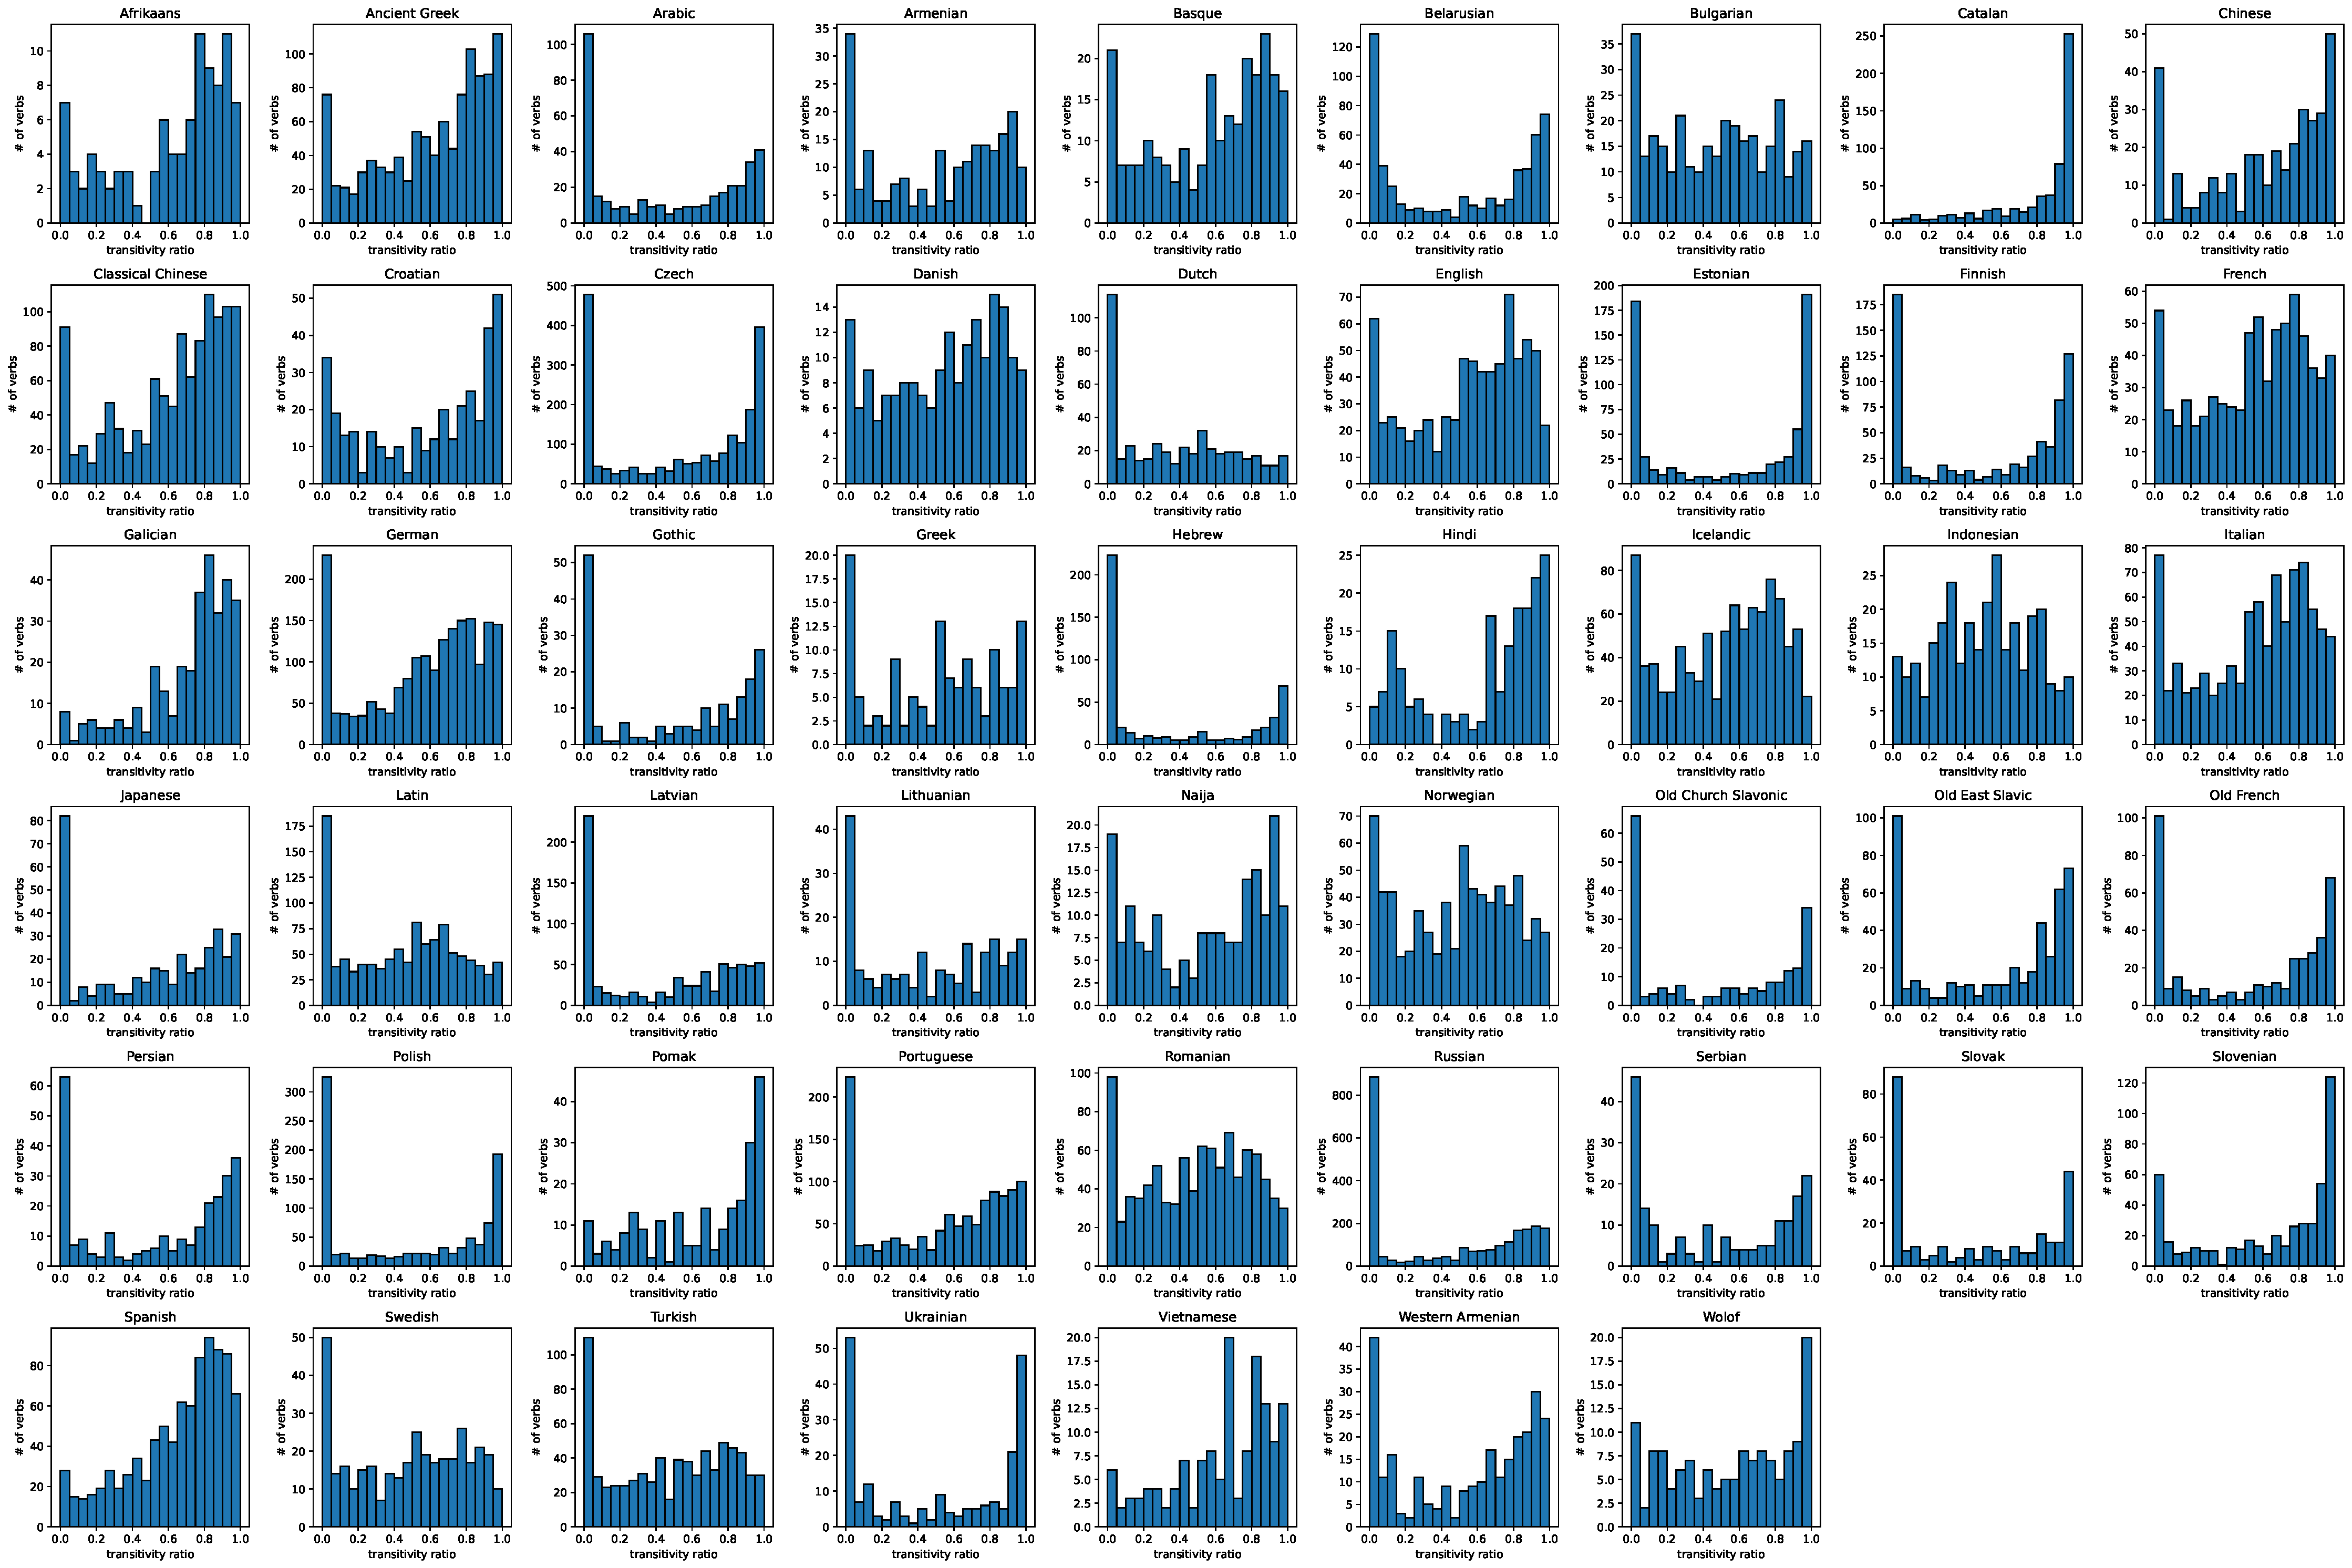
\includegraphics[width=\textwidth]{figures/verb_dist_by_transitivity.pdf}
  \caption{Histograms showing the binned distributions of verbs according to their transitivity ratio in different languages}
  \label{fig:verb_dist_transitivity}
\end{sidewaysfigure}

Most distributions are bimodal with peak at both ends, which supports the overall cross-lingual validity of a binary conception of transitivity. But exceptions abound as well, among others Indonesian (unimodal with peak in the middle), Catalan, Galician, Spanish (unimodal with peak on right). And even between the bimodal distributions, they are notably rarely symmetric, with differing levels of skew towards either end. 

\subsection{Genetic and areal patterns in transitivity}

\begin{table}[ht]
    \centering
    \small
    \begin{subtable}[c]{\textwidth}
      \centering
      \begin{tabular}{lrr|lrr}
        \toprule
        Language & \# Verbs & Tr. verb \% & Language & \# Verbs & Tr. verb \% \\
        \midrule
        Catalan & 628 & 99.2\% & Maltese & 78 & 55.1\% \\
        Galician & 341 & 97.7\% & Hebrew & 536 & 58.4\% \\
        Urdu & 69 & 97.1\% & Hungarian & 73 & 64.4\% \\
        Hindi & 207 & 97.1\% & Russian & 2583 & 65.0\% \\
        Spanish & 948 & 96.9\% & Slovak & 284 & 66.5\% \\
        Indonesian & 330 & 96.7\% & Uyghur & 93 & 66.7\% \\
        Vietnamese & 156 & 95.5\% & Coptic & 128 & 68.0\% \\
        French & 735 & 94.8\% & Old Church Slavonic & 223 & 68.6\% \\
        Gheg & 50 & 94.0\% & Polish & 1080 & 68.8\% \\
        Danish & 212 & 93.9\% & Bambara & 50 & 70.0\% \\
        English & 773 & 93.4\% & Erzya & 87 & 70.1\% \\
        Afrikaans & 119 & 93.3\% & Latvian & 794 & 71.2\% \\
        Norwegian & 765 & 92.9\% & Gothic & 201 & 73.1\% \\
        Basque & 255 & 92.9\% & Old French & 444 & 74.1\% \\
        Ancient Greek & 1127 & 92.7\% & Faroese & 117 & 74.4\% \\
        \dots & \dots & \dots & \dots & \dots & \dots \\
        \bottomrule
      \end{tabular}
      \caption{by transitive verb percentage}
      \label{tab:most_tr_by_verb_percentage}
    \end{subtable}\\
    \begin{subtable}[c]{\textwidth}
      \centering
      \begin{tabular}{lrr|lrr}
        \toprule
        Language & \# Verbs & Token tr. & Language & \# Verbs & Token tr. \\
        \midrule
        Akkadian & 76 & 75.9\% & Scottish Gaelic & 53 & 16.2\% \\
        Catalan & 628 & 75.9\% & Irish & 108 & 30.8\% \\
        Galician & 341 & 70.5\% & Maltese & 78 & 31.7\% \\
        Afrikaans & 119 & 65.3\% & Faroese & 117 & 32.6\% \\
        Urdu & 69 & 65.2\% & Japanese & 395 & 33.4\% \\
        Gheg & 50 & 64.8\% & Hebrew & 536 & 33.5\% \\
        Vietnamese & 156 & 64.8\% & Polish & 1080 & 34.0\% \\
        Thai & 77 & 64.7\% & Uyghur & 93 & 34.1\% \\
        Classical Chinese & 1192 & 63.8\% & Erzya & 87 & 36.0\% \\
        Pomak & 244 & 62.1\% & Russian & 2583 & 37.4\% \\
        Spanish & 948 & 61.1\% & Dutch & 497 & 37.5\% \\
        Hindi & 207 & 60.8\% & Latvian & 794 & 37.8\% \\
        Chinese & 380 & 60.7\% & North Sami & 76 & 38.2\% \\
        Xibe & 74 & 58.8\% & Serbian & 214 & 38.4\% \\
        Ancient Greek & 1127 & 58.5\% & Arabic & 407 & 39.7\% \\
        \dots & \dots & \dots & \dots & \dots & \dots \\
        \bottomrule
      \end{tabular}
      \caption{by token-level transitivity ratio}
      \label{tab:most_tr_by_token_mean}
    \end{subtable}
    \caption{Most and least transitive languages by different metrics}
    \label{tab:most_tr_languages}
  \end{table}

Tab.~\ref{tab:most_tr_by_verb_percentage} and \ref{tab:most_tr_by_token_mean} list the most and least `transitive' languages in our study, respectively according to the transitive verb percentage and the token-level transitivity ratio. Recall that token-level transitivity ratios are favored over lexeme-level ones for cross-lingual comparison.

Among the most transitive languages are Romance (Catalan, Spanish, French, Galician) and Germanic (German, Norwegian, English, Danish) languages of Europe, Sinitic languages (Chinese, Classical Chinese, particularly when measured by token-level transitivity ratio), Indonesian, Hindi. On the opposite end of the spectrum are Hebrew, Irish, Japanese, as well as Baltic (Lithuanian, Latvian) and Slavic (Slovak, Russian, Polish) languages, which have the lowest transitivity ratios.

\begin{sidewaysfigure}[ht]
  \centering
  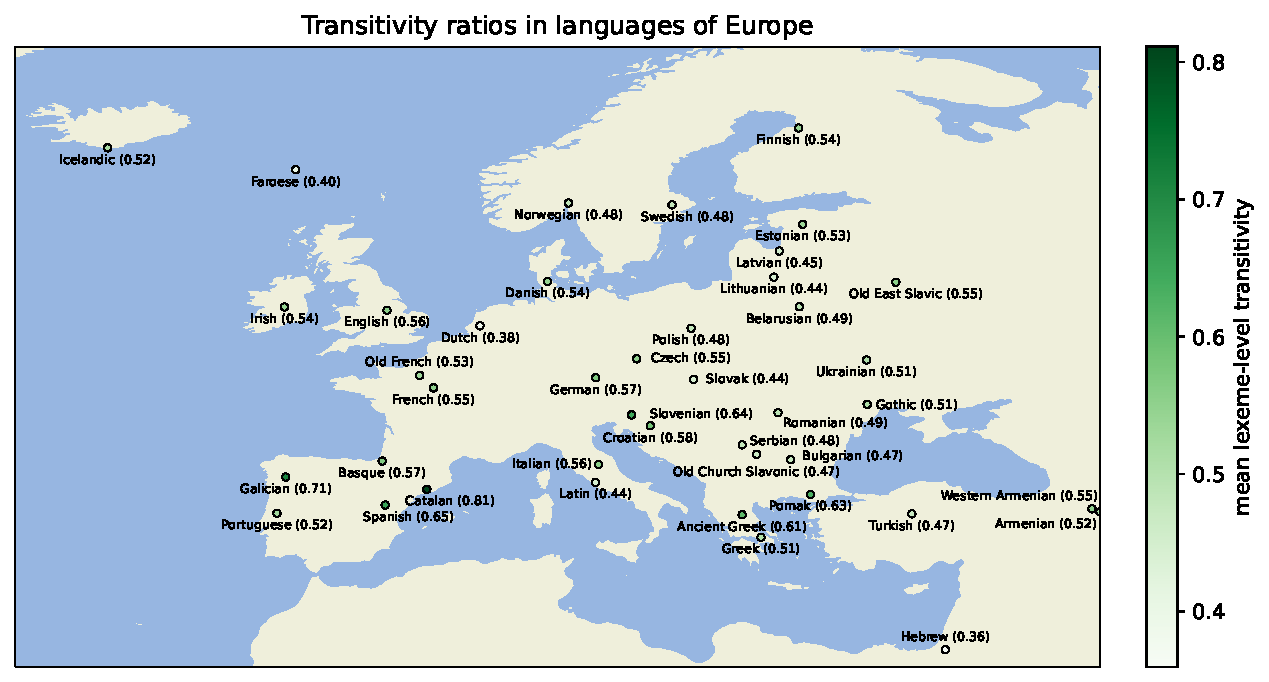
\includegraphics[width=\textwidth]{figures/transitivity_europe.pdf}
  \caption{Mean transitivity ratios in languages of Europe}
  \label{fig:transitivity_europe}
\end{sidewaysfigure}

To look at any potential areal patterns in transitivity, the token-level transitivity ratio results for European languages are also mapped in Fig.~\ref{fig:transitivity_europe}. (A less Eurocentric study of areal patterns is unfortunately difficult for the lack of enough language samples in the UD.) A particularly high transitivity area can be observed in the Iberian peninsular as well as another relatively high transitivity area in the Balkans, in contrast to eastern and northern Europe with lower transitivity.

Where the languages overlap, these observations match well with those from \citet{say2014}'s survey of transitivity in European languages (as measured by the percentage of verbs that are transitive from a fixed list), who observed high transitivity areas in western Europe except Irish and south-western Balkans, and a corresponding low transitivity area in eastern Europe.

% Dutch appears to be a special case in several ways. \todo{case study: Dutch - divergence btwn two metrics, maybe due to ergative verbs? and diff btwn Dutch vs Afrikanns - significant grammatical differences?}

% diff between tr. verb -> token-level tr. ratio reflects also the fact that tr. verbs can often be used intransitively
% how "free" a language is to use tr. verb  intr./vice versa is another interesting further study 
